\secnumbersection{DEFINICIÓN DEL PROBLEMA}

\subsection{La Web Semántica, RDF y SPARQL}

La Web Semántica es un conjunto de extensiones para la \textit{World Wide Web}, desarrolladas por el \textit{World Wide Web Consortium (W3C)}, las cuales buscan permitir que la información disponible en la Web pueda ser procesada de forma eficiente por máquinas \cite{berners2001semantic}. Para lograr esto, la web semántica propone agregar a la información ya existente metadatos semánticos para que estos puedan ser procesados por agentes inteligentes, los cuales, obtendrán esta información sin operadores humanos. Estos metadatos pueden ser descritos utilizando múltiples estándares existentes, uno de ellos es el \textit{Resource Description Framework (RDF)} \cite{world2014rdf}.

\textit{RDF} nos permite describir relaciones a través de trios del tipo ``\textit{Sujeto - Predicado - Objeto}'', los cuales, pueden ser representados de manera grafica a través de grafos. Un ejemplo de esto se puede apreciar en la figura \ref{fig:rdf-graph1}. En el grafo, el sujeto y el objeto son representados por vertices y el predicado, la relación entre ellos, se representa con una arista.

Cada uno de los elementos del trio corresponde a un objeto en la Web, los cuales, son identificados por Identificadores de Recursos Uniforme\footnote{Del ingles \textit{Uniform Resource Identifiers (URIs)}.}. Un ejemplo de estas \textit{URIs} es \href{http://www.wikidata.org/entity/Q1}{http://www.wikidata.org/entity/Q1} la cual identifica a ``El Universo'' en el repositorio de datos Wikidata. Sin embargo, existen ocasiones en las que no buscamos definir todo el grafo de forma constante y dejar determiados vertices o aristas en blanco, de forma tal que el grafo que estamos construyendo sea un grafo incompleto. Esto nos introduce al concepto de una variable en un grafo incompleto.


\begin{figure}[ht]
    \centering
    \includesvg[width=0.95\linewidth]{rdf-graph.svg}
    \caption{Un grafo \textit{RDF} básico.} Los nodos \textit{Subject} y
    \textit{Object} están conectados a través de la relación \textit{Predicate}.
    Fuente: \textit{RDF 1.1 Concepts and Abstract Syntax. World Wide Web
    Consortium}.
    \label{fig:rdf-graph1}
\end{figure}

Un conjunto de multiples trios nos permite construir grafos más complejos, los cuales, en conjunto con vertices variables nos permiten definir patrones de grafos, los cuales, al asignar valores concretos en sus variables generan una solución al patron representado. Un ejemplo de estos patrones se puede apreciar en la figura \ref{fig:rdf-graph-pattern-drug}.

\begin{figure}[ht]
    \centering
    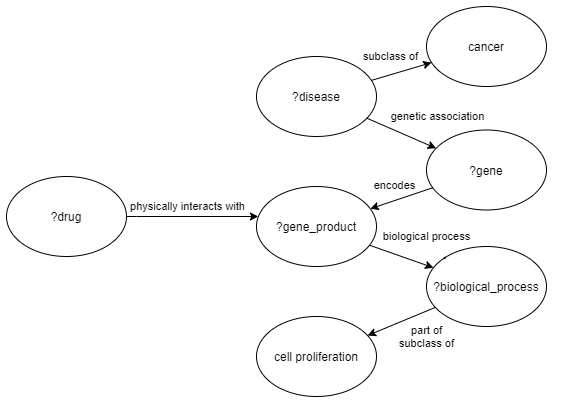
\includegraphics[width=0.95\linewidth]{graph-pattern-drug.png}
    \caption{Un grafo que representa un patron complejo.} Aquellos grafos que son solución de este patron, corresponden a aquellos medicamentos para el cáncer que afecta a los genes relacionados con la proliferación celular. Fuente: Elaboración propia.
    \label{fig:rdf-graph-pattern-drug}
\end{figure}

Estos grafos incompletos pueden ser presentados a bases de datos orientadas a grafos para ser completados a través de consultas con datos que esta base de datos en particular contiene, obteniendo así, soluciones que cumplen con el patron presentado. Existen multiples motores de bases de datos orientadas a grafos, en este trabajo nos centraremos en el repositorio de datos \textit{Wikidata} \cite{erxleben2014introducing} y su motor de busqueda \textit{Wikidata Query Service}\footnote{\href{https://query.wikidata.org/}{https://query.wikidata.org/}}.

En un ejemplo concreto, podemos obtener soluciones para el grafo de la figura \ref{fig:rdf-graph-pattern-drug} en \textit{Wikidata} a través de la consulta \textit{SPARQL} que se puede apreciar en la figura \ref{code:sparql-query-drug}. \textit{SPARQL (SPARQL Protocol And RDF Query Language)} corresponde al lenguaje estandarizado para describir consultas a repositorios de datos RDF orientados a grafos.

\subsection{Dificultades al utilizar SPARQL}

En base a todo lo anterior podemos notar lo siguiente: Para utilizar \textit{SPARQL} y obtener información util y relevante desde un repositorio \textit{RDF}, como usuarios, necesitamos dos cosas.

\begin{enumerate}
    \item Conocer la sintaxis del lenguaje para consultas \textit{SPARQL}
    \item Conocer la estructura de los elementos disponibles en el repositorio \textit{RDF}
\end{enumerate}

\begin{figure}[ht]
    \begin{lstlisting}[language=SPARQL]
    PREFIX wdt: <http://www.wikidata.org/prop/direct/>
    PREFIX wd: <http://www.wikidata.org/entity/>
        
    SELECT DISTINCT ?biological_process ?drug ?gene ?disease WHERE {
        ?gene_product wdt:P682 ?biological_process .
        ?biological_process (wdt:P361|wdt:P279)* wd:Q14818032 .
        ?drug wdt:P129 ?gene_product .
        ?gene wdt:P688 ?gene_product .
        ?disease wdt:P2293 ?gene .
        ?disease wdt:P279* wd:Q12078 .
    }
    \end{lstlisting}
    \caption{Consulta \textit{SPARQL} generada por el grafo incompleto de la figura \ref{fig:rdf-graph-pattern-drug}.} Fuente: Elaboración propia.
    \label{code:sparql-query-drug}
\end{figure}

Es bastante complicado cumplir estos prerequisitos si nuestros usuarios no tienen experiencia brevia en estas materias. Por lo tanto, para apoyar a nuestros usuarios en el proceso de cumplir sus necesidades se han desarrollado herramientas y plataformas que facilitan la construcción de consultas y la exploración de las entidades en las bases de datos \textit{RDF} como por ejemplo, \textit{RDFExplorer} \cite{vargas2019rdf}, \textit{Tabulator} \cite{berners2006tabulator} , \textit{Explorator} \cite{araujo2009experimenting}, \textit{DBpedia Atlas} \cite{valsecchi2015dbpedia}, \textit{RDF Visualizer} \cite{sayers2004node}, \textit{SPARQL Assist} \cite{mccarthy2012sparql} o \textit{YASGUI} \cite{rietveld2017yasgui}.

En este trabajo hemos decidido utilizar \textit{RDFExplorer} en base a las siguientes caracteristicas.

\begin{itemize}
    \item Facilidad de uso en su interfaz.
    \item Construcción interactiva de consultas \textit{SPARQL}.
    \item Navegación de las entidades disponibles en la base de datos \textit{RDF}.
    \item Generación de resultados parciales.
    \item Código fuente disponible y abierto \cite{vargas2019rdfrepo}.
    \item Disponible a través de una interfaz Web.
\end{itemize}

Una vista de su interfaz se puede apreciar en la figura \ref{fig:rdfexplorer}.

\begin{figure}
    \centering
    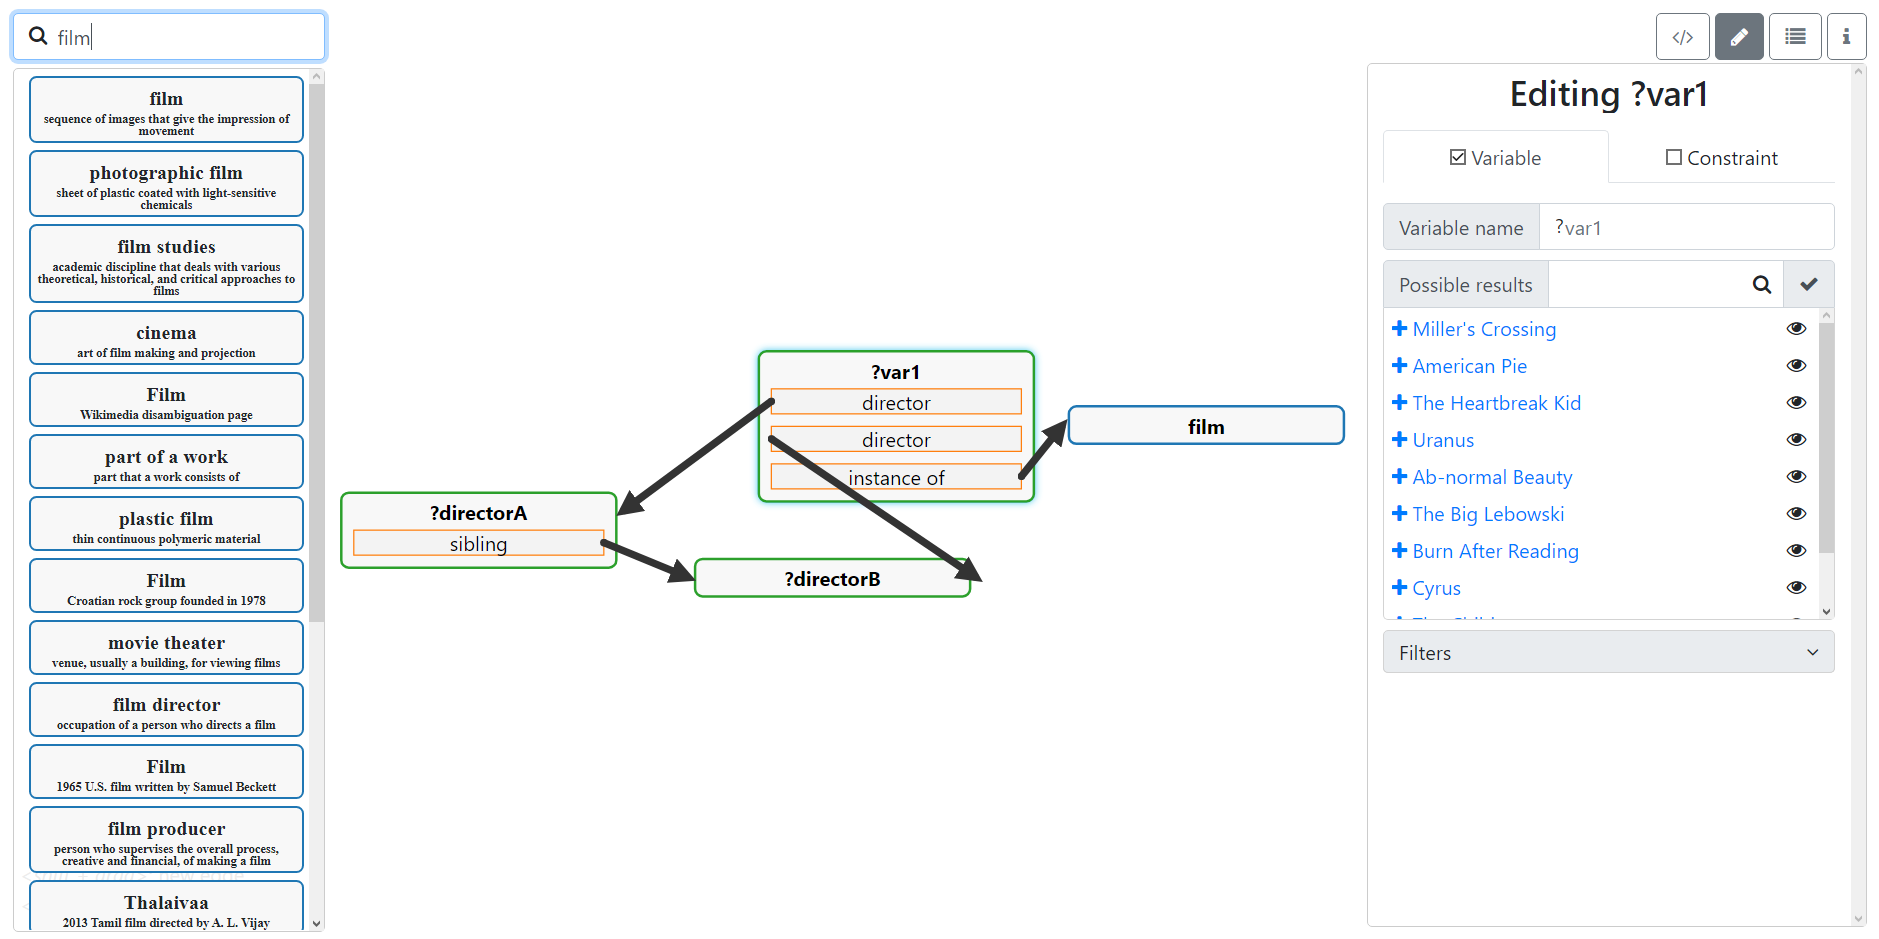
\includegraphics[width=\linewidth]{rdfexplorer.png}
    \caption{RDFExplorer, construcción de una consulta \textit{SPARQL}.} Obtiene el conjunto de aquellas películas que han sido dirigidas por hermanos. A la derecha, un conjunto de posibles resultados. Fuente: Elaboración propia.
    \label{fig:rdfexplorer}
\end{figure}

Sin embargo, aun cuando utilizamos herramientas como \textit{RDFExplorer} debemos tener algún grado de conocimiento sobre las propiedades de las entidades disponibles en nuestro repositorio \textit{RDF}. Para apoyar en esta tarea, podemos generar recomendaciones o sugerencias sobre los posibles resultados o soluciones de un grafo incompleto determiado. Esto es similar a las herramientas y funcionalidades para el autocompletado en procesadores de texto o entornos de desarrollo integrados \cite{bruch2009learning}.

\subsection{Generación de sugerencias}

En la actualidad, existen soluciones y herramientas que nos permiten obtener recomendaciones en base a consultas \textit{SPARQL} incompletas. Ejemplos de estas soluciones son \textit{Gosparqled} \cite{campinas2014live}, \textit{LinkedWiki editor} \cite{rafes2018designing}, \textit{SPARKLIS} \cite{ferre2017sparklis}, \textit{SPACE} \cite{kramer2013space} y \textit{SPARQLforHumans} \cite{parra2020autocompletion}. De las alternativas mencionadas, una tiene una importrante ventaja; \textit{SPARQLforHumans} se encuentra integrado con \textit{RDFExplorer}.

\textit{SPARQLforHumans} pareciera ser la solución a este problema, sin embargo, tiene ciertos problemas importantes descritos por sus autores.

\begin{itemize}
    \item El tiempo necesario para iniciar el software puede tomar hasta $109$ horas.
    \item Una vez iniciado el software, sus resultados son inmediatamente obsoletos. Esto, debido a que en \textit{Wikidata} pueden llegar a ocurrir $200.000$ cambios por día.
    \item El hecho de estar diseñado para soportar distintos tipos de repositorios \textit{RDF} no permite realizar optimizaciones importantes a su rendimiento.
\end{itemize}

En nuestro proyecto, vemos estos problemas como oportunidades de mejorar el rendimiento general del sistema propuesto por \textit{SPARQLforHumans}.

\subsection{Objetivos}

En base a todo lo expuesto anteriormente, en este trabajo buscamoos replicar y lograr las mismas funcionalidades generadas por el proyecto \textit{SPARQLforHumans} implementando las siguientes mejoras.

\begin{itemize}
    \item Reducir el tiempo de procesamiento para los volcados de la base de datos de \textit{Wikidata} durante el proceso de inicio del software.
    \item Implementar un mecanismo de actualización constante con los datos obtenidos directamente desde \textit{Wikidata}.
\end{itemize}

Además, vamos a definir las siguientes restricciones para nuestra solución:

\begin{itemize}
    \item Utilizaremos datos desde el repositorio \textit{RDF} \textit{Wikidata}.
    \item Utilizaremos componentes gratuitos y de código abierto para nuestro desarrollo de software.
\end{itemize}

Por ultimo, podemos definir nuestro objetivo general y objetivos especificos.

\subsubsection{Objetivo general}

Analizar, diseñar e implementar una nueva arquitectura para el proyecto \textit{SPARQLforHumans}, utilizando exclusivamente componentes de código abierto.

\subsubsection{Objetivos específicos}

\begin{itemize}
    \item Revisar y evaluar la arquitectura actual del proyecto \textit{SPARQLforHumans}.
    \item Diseñar la arquitectura del sistema utilizando solamente componentes de código abierto.
    \item Implementar la arquitectura propuesta.
    \item Evaluar el rendimiento de la solución implementada.
\end{itemize}
